\documentclass[prd,showpacs,twocolumn]{revtex4-1}
%\documentclass[12pt]{iopart}
\usepackage{graphicx}% Include figure files
\usepackage{dcolumn}% Align table columns on decimal point
\usepackage{bm}% bold math
%\nofiles
\begin{document}
\title{Linear relationship between frequency and energy of a wave train}
\author{Peifeng Wang}
\email{peifeng\_w@yahoo.com}
\author{Peilei Wang}
\address{Guanghua Road 1\#, 34-1-3-5, Yanta District, Xi'an, Shaanxi, P. R. China 710075}
\address{Mijiaqiao 34-1-3-5, Xi'an, Shaanxi, P. R. China 710075}
\begin{abstract}
We demonstrate that, under Lorentz transformation, the frequency and the energy of an electromagnetic wave train form a linear relationship, emulating the equation of photon energy $E=\hbar\omega$. This shows that wave-particle duality of light is compatible under space time transformation.
\end{abstract}
\pacs{03.50.De}
\maketitle

Wave-particle duality is one of the most fundamental characters of quanta and is revealed by the linear dependence between energy and frequency of a particle. In most cases, treatment of physical entities deals only with one of the properties at a time. For photon, one of the basic elementary particle, the wave property is studied by examining the few-cycle light pulses \cite{Salieres, Jones, Hentschel, Nisoli, Paulus}, while the particle property is learned by investigating the interaction of photon with other particles \cite{Gluck, Donnachie, Belitsky, Baba, Fiore}.

Here, we demonstrate that under Lorentz transformation, the energy of an electromagnetic wave train is linearly dependent on the frequency of that same wave train. Our model is based on the observation that in electrodynamics, space time transformation can simultaneously lead to both Doppler effect and a change of magnitude of electromagnetic (EM) fields. Consequently, there exists a relationship between Doppler frequency shift and the energy flow change of plane EM wave train due to space time transformation. It turns out that this relationship, resulting completely from wave theory, is linear, emulating the equation of photon energy $E=\hbar\omega$.

For a plane EM wave train of duration $\Delta t$, the time rate of energy flow through unit area is related to the fields $(\mathbf{E}, \mathbf{B})$ of the wave by Poynting's theorem
\begin{eqnarray}
\mathbf{S}=\frac{1}{\mu}\mathbf{E}\times\mathbf{B}
\end{eqnarray}
then the total energy flow of the wave train through unit area is
\begin{eqnarray}
\mathbf{P}=\mathbf{S}\Delta t
\end{eqnarray}

The values of $(\mathbf{E}, \mathbf{B})$ are both dependent on the selected reference frame. The transformation of electromagnetic fields from reference frame $F$ to frame $F'$ moving with velocity $\mathbf{v}$ relative to $F$ are \cite{Jackson}
\begin{eqnarray}
&&[\mathbf{E'}]_{\mathbf{x'},t'}=[\gamma(\mathbf{E}+\beta\times \mathbf{B})-\frac{\gamma^2}{\gamma+1}\mathbf{\beta}(\mathbf{\beta}\cdot \mathbf{E})]_{\mathbf{x},t}\nonumber\\
&&[\mathbf{B'}]_{\mathbf{x'},t'}=[\gamma(\mathbf{B}-\beta\times \mathbf{E})-\frac{\gamma^2}{\gamma+1}\mathbf{\beta}(\mathbf{\beta}\cdot \mathbf{B})]_{\mathbf{x},t}\nonumber\\
&&\beta=\frac{\mathbf{v}}{c},\gamma=\frac{1}{\sqrt{1-\beta^2}}
\label{eqn:E1B1}
\end{eqnarray}

The above transformation of fields $\mathbf{E}, \mathbf{B}$ will inevitably lead to variation of $(\mathbf{S}, \mathbf{P})$ in different frames.

On the other hand, viewed from different frames, the frequency of EM wave follows the formulas of relativistic Doppler effect
\begin{eqnarray}
\omega'&&=\gamma\omega(1-\beta\cos\theta)\nonumber\\
\tan\theta'&&=\frac{\sin\theta}{\gamma(\cos\theta-\beta)}
\label{eqn:Doppler}
\end{eqnarray}
$\theta$ is the angle between $\beta$ and the wave propagation direction $\mathbf{k}$ observed in frame $F$.

We will show that for any given plane EM wave train under Lorentz transformation, $|\mathbf{P}'|=\mathbf{E}'\times\mathbf{B}'\Delta t'/\mu$ varies in the same way as $\omega'$. Consequently
\begin{eqnarray}
|\mathbf{P}'|\propto\omega'
\label{eqn:main1}
\end{eqnarray}
Throughout our discussion, the Gaussian units are used, so for the electric and magnetic fields $(\mathbf{E}, \mathbf{B})$ in a plane EM wave, we have
\begin{eqnarray}
|\mathbf{E}|=|\mathbf{B}|
\label{eqn:convention}
\end{eqnarray}

The primed quantities are evaluated at $(\mathbf{x'},t')$ in frame $F'$, while the unprimed quantities are evaluated at $(\mathbf{x},t)$ in frame $F$. $(\mathbf{x'},t')$ and $(\mathbf{x},t)$ are related by Lorentz transformation
\begin{eqnarray}
t'&&=\gamma(t-\beta\cdot\mathbf{x})\nonumber\\
\mathbf{x'}&&=\mathbf{x}+\frac{\gamma-1}{\beta^2}\beta(\beta\cdot\mathbf{x})-t\gamma\beta
\end{eqnarray}

To prove eqn. (\ref{eqn:main1}), we first discuss two special cases, 1) $\beta$ is parallel to the propagation direction $\mathbf{k}$. 2) $\beta$ is perpendicular to propagation direction $\mathbf{k}$. Then we generalize to the situation of arbitrary angle $\theta$ between $\beta$ and $\mathbf{k}$.

\begin{figure}
\center
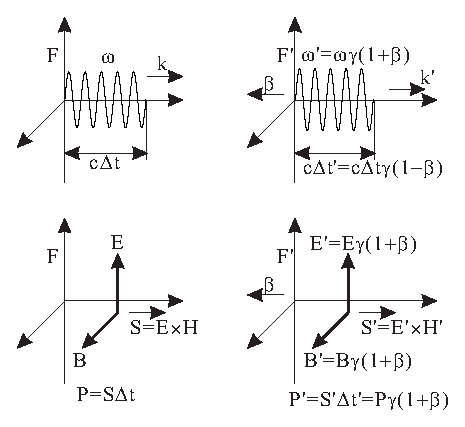
\includegraphics{Graph1.eps}
\caption{$\beta$ is parallel to wave propagation $\mathbf{k}$ in frame $F$. The left column shows the wave train and corresponding fields $\mathbf{E}, \mathbf{B}$ in frame $F$, the right column shows the wave train and corresponding fields $\mathbf{E}', \mathbf{B}'$ in frame $F'$}
\label{fig:P}
\end{figure}

For $\beta$ parallel to the propagation direction $\mathbf{k}$ in frame $F$, as shown in fig. \ref{fig:P}, $\beta\cdot\mathbf{E}=0, \beta\cdot\mathbf{B}=0$, then from eqn. (\ref{eqn:E1B1}), fields in frame $F'$ are
\begin{eqnarray}
\mathbf{E'}=\gamma(\mathbf{E}+\beta\times \mathbf{B})\nonumber\\
\mathbf{B'}=\gamma(\mathbf{B}-\beta\times \mathbf{E})
\end{eqnarray}
then with eqn. (\ref{eqn:convention})
\begin{eqnarray}
\mathbf{E'}=\gamma(1+\beta)\mathbf{E}\nonumber\\
\mathbf{B'}=\gamma(1+\beta)\mathbf{B}
\label{eqn:fP}
\end{eqnarray}

Since the magnetic permeability $\mu$ is invariant in any frame, the Poynting vector observed in frame $F'$ is
\begin{eqnarray}
\mathbf{S}'=\frac{\mathbf{E}'\times\mathbf{B}'}{\mu}=\gamma^2(1+\beta)^2\frac{\mathbf{E}\times\mathbf{B}}{\mu}=\gamma^2(1+\beta)^2\mathbf{S}
\end{eqnarray}

The duration of the wave train in frame $F'$ is
\begin{eqnarray}
\Delta t'=\gamma(1-\beta)\Delta t
\end{eqnarray}
using the identity
\begin{eqnarray}
\gamma(1-\beta)=\frac{1}{\gamma(1+\beta)}
\end{eqnarray}
we arrive at
\begin{eqnarray}
\Delta t'=\frac{1}{\gamma(1+\beta)}\Delta t
\label{eqn:tP}
\end{eqnarray}

The energy flow of wave train through unit area observed in frame $F'$ is
\begin{eqnarray}
\mathbf{P}'=\mathbf{S}'\Delta t'=\gamma^2(1+\beta)^2\mathbf{S}\frac{1}{\gamma(1+\beta)}\Delta t=\gamma(1+\beta)\mathbf{P}
\label{eqn:PP}
\end{eqnarray}

On the other hand, the Doppler frequency shift in eqn. (\ref{eqn:Doppler}) at $\theta=\pi$ is
\begin{eqnarray}
\omega'&&=\gamma(1+\beta)\omega
\label{eqn:OP}
\end{eqnarray}

Eqn. (\ref{eqn:PP}) and (\ref{eqn:OP}) show an identical variation of $\mathbf{P}$ and $\omega$ under Lorentz transformation. Eqn. (\ref{eqn:main1}) comes as
\begin{eqnarray}
\frac{|\mathbf{P}'|}{\omega'}&&=\frac{|\mathbf{P}|}{\omega}=const
\label{eqn:mainP}
\end{eqnarray}

In the case that $\beta$ is in the same direction of wave propagation $\mathbf{k}$ and $\theta=0$, we just need to replace $\beta$ in the above equation with $-\beta$, and the same result (\ref{eqn:mainP}) yields.

\begin{figure}
\center
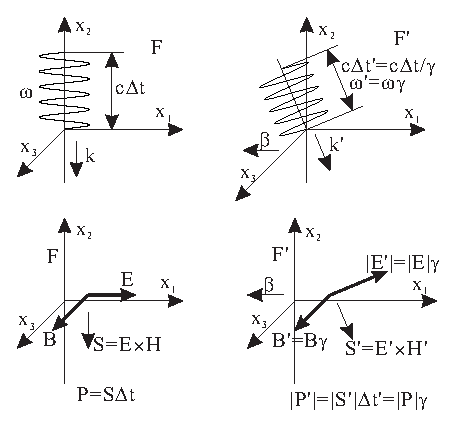
\includegraphics{Graph2.eps}
\caption{$\beta$ is perpendicular to wave propagation $\mathbf{k}$ in frame $F$. The left column shows the wave train and corresponding fields $\mathbf{E}, \mathbf{B}$ in frame $F$, the right column shows the wave train and corresponding fields $\mathbf{E}', \mathbf{B}'$ in frame $F'$. Note that the direction of wave propagation and Poynting vector differs in the two frames.}
\label{fig:V}
\end{figure}

Next is the calculation for $\beta$ perpendicular to the propagation direction $\mathbf{k}$. For simplicity, we assume the electric field $\mathbf{E}$ parallel to $\beta$. The explicit form of eqn. (\ref{eqn:E1B1}) are
\begin{eqnarray}
E_1'=E_1\nonumber\\
E_2'=\gamma(E_2-\beta B_3)\nonumber\\
E_3'=\gamma(E_3+\beta B_2)\nonumber\\
B_1'=B_1\nonumber\\
B_2'=\gamma(B_2+\beta E3)\nonumber\\
B_3'=\gamma(B_3-\beta B2)
\end{eqnarray}

From the configuration shown in fig. \ref{fig:V}, the fields observed in frame $F'$ are
\begin{eqnarray}
E_1'=E_1\nonumber\\
E_2'=-\gamma\beta B_3\nonumber\\
E_3'=0\nonumber\\
B_1'=0\nonumber\\
B_2'=0\nonumber\\
B_3'=\gamma B_3
\end{eqnarray}
with eqn. (\ref{eqn:convention}), it follows
\begin{eqnarray}
|\mathbf{E}'|=\gamma|\mathbf{E}|, |\mathbf{B}'|=\gamma|\mathbf{B}|
\label{eqn:fV}
\end{eqnarray}

The magnitude of Poynting vector is
\begin{eqnarray}
|\mathbf{S}'|=\frac{1}{\mu}|\mathbf{E}'\times\mathbf{H}'|=\gamma^2\frac{1}{\mu}|\mathbf{E}\times\mathbf{H}|=\gamma^2|\mathbf{S}|
\end{eqnarray}

The duration of the wave train is
\begin{eqnarray}
\Delta t'=\Delta t/\gamma
\label{eqn:tV}
\end{eqnarray}

Then in frame $F'$, energy flow of wave train through unit area is
\begin{eqnarray}
|\mathbf{P}'|=|\mathbf{S}'\Delta t'|=\gamma|\mathbf{P}|
\end{eqnarray}

On the other hand, eqn. (\ref{eqn:Doppler}) shows that the Doppler frequency shift at $\theta=\pi/2$ is
\begin{eqnarray}
\omega'&&=\gamma\omega
\label{eqn:DopplerV}
\end{eqnarray}

Again, an identical variation of $|\mathbf{P}|$ and $\omega$ under Lorentz transformation emerges, and eqn. (\ref{eqn:main1}) follows as
\begin{eqnarray}
\frac{|\mathbf{P}'|}{\omega'}&&=\frac{|\mathbf{P}|}{\omega}=const
\label{eqn:mainV}
\end{eqnarray}

Eqn. (\ref{eqn:mainP}) and (\ref{eqn:mainV}) are proofs of eqn. (\ref{eqn:main1}) when the angle $\theta$ between $\beta$ and wave propagation $\mathbf{k}$ is either $0, \pi$ or $\pi/2$. In the case that $\theta$ is arbitrary, the calculation can be done in the following way. By decomposing $\beta$ into a component $\beta_p$ parallel to $\mathbf{k}$ and a component $\beta_v$ vertical to $\mathbf{k}$, we can compute the total effect as a superposition of the parallel case of $\beta_p$ and the vertical case of $\beta_v$. Therefore, eqn. (\ref{eqn:main1}) holds true for all cases.

Unlike other particles, which may appear at rest in some specific reference frame, the speed of EM wave train is invariant in any frame. That is, all frames are equivalent in the observation of EM wave. Therefore, for any given wave train, the above equations show that the ratio between its frequency and energy flow through unit area remains constant independent of the reference frame in which the EM wave train is observed.

The proportional relationship between the frequency of a wave train and its energy flow emulates the equation of photon energy $E=\hbar\omega$. Furthermore, under Lorentz transformation, the frequency of an electromagnetic wave train is proportional to the magnitude of its fields. This can be derived from eqn. (\ref{eqn:fP}), (\ref{eqn:OP}) and eqn. (\ref{eqn:fV}), (\ref{eqn:DopplerV})
\begin{eqnarray}
\omega\propto|\mathbf{E}|, \omega\propto|\mathbf{B}|
\end{eqnarray}

From wave theory and Fourier analysis, a finite length wave train of $N$ cycles has a frequency spectrum breadth $\Delta\omega$.
\begin{eqnarray}
\frac{\Delta\omega}{\omega}=\frac{1}{2N}
\label{eqn:Domega}
\end{eqnarray}

If the time duration $\Delta t$ of a wave train is interpreted as the uncertainty in time and the spectrum breadth $\Delta\omega$ as the uncertainty in frequency, we have
\begin{eqnarray}
\Delta\omega \Delta t=\frac{\omega \Delta t}{2N}=\pi
\label{eqn:DoDt}
\end{eqnarray}

With eqn. (\ref{eqn:main1}), the following relationship holds for a give electromagnetic wave train when observed in different frames.
\begin{eqnarray}
|\Delta \mathbf{P}| \Delta t=const
\label{eqn:t}
\end{eqnarray}

This emulates the uncertainty principle in quantum theory
\begin{eqnarray}
\Delta E \Delta t=\hbar\Delta\omega\Delta t>\frac{h}{2}\nonumber\\
\Delta p \Delta x=\frac{\hbar\Delta\omega}{c}c\Delta t>\frac{h}{2}
\label{eqn:uncertainty}
\end{eqnarray}

In conclusion, we have shown that under space time transformation, Doppler frequency shift $\omega$ and the energy flow $|\mathbf{P}|$ of EM wave train are related linearly, emulating the equation of photon energy $E=\hbar\omega$. If a wave train has a ratio $E/\omega=\hbar$, then it has the same ratio in all frames, while its $E$ and $\omega$ varies respectively. This proportional dependency reveals that the model of photon holds under space time transformation. Our derivation is completely from Lorentz transformation and Doppler effect. Conversely, the linear relationship between the energy and frequency of photon implies that the speed of light is constant.

It is also noted that 1) the number of cycles of a wave train remains unchanged in different frames and 2) an observed $\omega'$ photon(wave train) resulted from Doppler shift of an `original' $\omega$ photon is indistinguishable from an `original' $\omega'$ photon. It is then speculated that all photons contain the same number of cycles.

%\ack
%I am grateful to my family for their support and encouragement.

\begin{thebibliography}{}
\label{sec:TeXbooks}
\bibitem{Salieres} P. Salieres, P. Antoine, A. de Bohan, and M. Lewenstein, \emph{Phys. Rev. Lett.} 81, 5544 (1998).
\bibitem{Jones} D. J. Jones, S. A. Diddams, J. K. Ranka, A. Stentz, R. S. Windeler, J. L. Hall, and S. T. Cundiff, \emph{Science} 288, 635 (2000).
\bibitem{Hentschel} M. Hentschel, R. Kienberger, Ch. Spielmann, G. A. Reider, N. Milosevic, T. Brabec, P. Corkum, U. Heinzmann, M. Drescher, and F. Krausz, \emph{Nature}(London) 414, 509 (2001).
\bibitem{Nisoli} M. Nisoli, G. Sansone, S. Stagira, S. De Silvestri, C.Vozzi, M. Pascolini, L. Poletto, P. Villoresi, and G. Tondello, \emph{Phys. Rev. Lett.} 91, 213905 (2003).
\bibitem{Paulus} G. G. Paulus, F. Lindner, H. Walther, A. Baltuska, E. Goulielmakis, M. Lezius, and F. Krausz, \emph{Phys. Rev. Lett.} 91, 253004 (2003).
\bibitem{Gluck} M. Gluck, E. Reya, and I. Schienbein, \emph{Phys. Rev. D} 63, 074008 (2001).
\bibitem{Donnachie} A. Donnachie, H. G. Dosch, \emph{Phys. Rev. D} 65, 014019 (2002).
\bibitem{Belitsky} A. V. Belitsky, D. Muller, and A. Kirchner, \emph{Nucl. Phys. B} 629, 323 (2002).
\bibitem{Baba} H. Baba, K. Sasaki, and T. Uematsu, \emph{Phys. Rev. D} 68, 054025 (2003).
\bibitem{Fiore} R. Fiore, A. Flachi, L. L. Jenkovszky, A. I. Lengyel, and V. K. Magas, \emph{Phys. Rev. D} 69, 014004 (2004).
\bibitem{Jackson} J. D. Jackson, \emph{Classical Electrodynamics}, 3rd edition, Wiley, NY (1998).
\end{thebibliography}
\end{document}

